\sectionSlide{Summary}{c++-logo}{0.9\paperheight}{b}


\slide{Key messages}{
    \Large 
    \enumstep{
        \item C++ had a \textbf{clear aim}, which made it popular: to \textbf{organize code better without the loss of efficiency} \\~\\
        \item C++ is even more popular now, because of new standards: \textbf{C++11} and \textbf{C++14} \\~\\
        \item In future C++ will be \textbf{one of the most popular programming languages} so it's worth learning
    }
}


\slide{Worth reading / watching}{
    \begin{thebibliography}{9}
        \setbeamertemplate{bibliography item}[online]
        \bibitem{Stroustrup} Bjarne Stroustrup -- \textit{The Evolution of C++ - Past, Present, and Future} \\
        {\scriptsize CppCon 2016 \\ \url{https://www.youtube.com/watch?v=_wzc7a3McOs}}
        \bibitem{Sutter} Herb Sutter -- \textit{One C++} \\
        {\scriptsize Going Native 2013 \\ \url{https://channel9.msdn.com/Events/GoingNative/2013/Keynote-Herb-Sutter-One-Cpp}} 
        \bibitem{Gregory} Kate Gregory -- \textit{Stop teaching C} \\
        {\scriptsize CppCon 2015 \\ \url{https://www.youtube.com/watch?v=YnWhqhNdYyk}}    
        \setbeamertemplate{bibliography item}[article]
        \bibitem{Stroustrup2} Bjarne Stroustrup -- \textit{A History of C++: 1979-1991} \\
        {\scriptsize \url{http://www.stroustrup.com/hopl2.pdf}}
        \setbeamertemplate{bibliography item}[book]
        \bibitem{Meyers} Scott Meyers -- \textit{Effective Modern C++}
    \end{thebibliography}
}


\slide{What now?}{
    \begin{block}{What now?}
        \itemstep{
            \item Look forward to C++17 and learn it
            \item Watch a lot of videos from C++ conferences
            \item Visit \url{isocpp.org}
        }
    \end{block}
}


\slide{Famous quotation}{
    \begin{columns}
    \begin{column}{0.7\textwidth}
        \begin{block}{}
            \begin{quotation}
                {\Large ``Learn C++. It's an investment.''}
            \end{quotation}
            \pause
            \rightline{{\rm --- Łukasz Ziobroń}}
        \end{block}    
    \end{column}
    \begin{column}{0.3\textwidth}
        \centering
        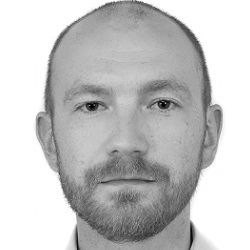
\includegraphics[height=100pt]{LukaszZiobron}
    \end{column}
    \end{columns}
}

%TODO: Sources

\imageSlide{keep-calm-and-ask-questions}